\documentclass[12pt]{article}
\linespread{2}
\usepackage{times}
\usepackage{pgfplots}
\pgfplotsset{compat = newest}
\usetikzlibrary{positioning, arrows.meta}
\usepgfplotslibrary{fillbetween}
\usepackage{amsmath}
           \begin{document} 
                  \begin{center}
                       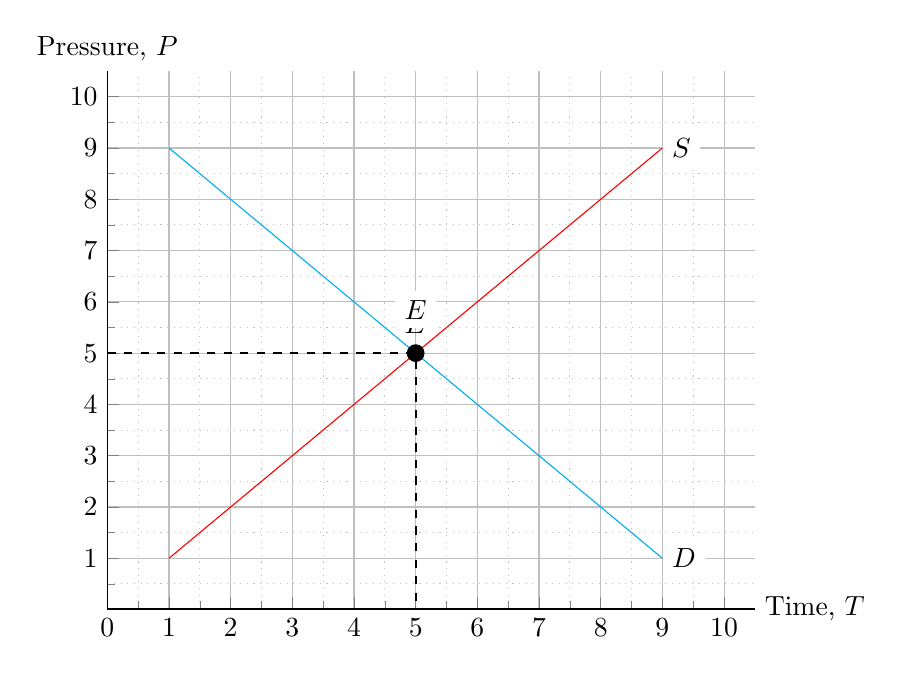
\begin{tikzpicture}
                            \begin{axis}[
                                         scale = 1.2,
                                         xmin = 0, xmax = 10.5,
                                         ymin = 0.01, ymax = 10.5,
                                         axis lines* = left,
                                         xtick = {0,1,2,3,4,5,6,7,8,9,10},
                                         ytick = {0,1,2,3,4,5,6,7,8,9,10},
                                         grid = both,
                                         minor tick num = 1,
                                         grid style = solid,
                                         minor grid style = dotted,
                                         clip = false,
]


% Supply and demand curves
                           \addplot[color = cyan] coordinates {(1, 9) (9, 1)};
                           \addplot[color = red] coordinates {(1, 1) (9, 9)};


% Dashed lines
                           \addplot[color = black, dashed, thick] coordinates {(0, 5) (5, 5)(5, 0)};



% Coordinate points
                           \addplot[color = black, mark = *, only marks, mark size = 3pt]
                            coordinates {(5, 5)};



% Labels
                              \node [right] at (current axis.right of origin) {Time, $T$};
                              \node [above] at (current axis.above origin) {Pressure, $P$};
                              \node [above] at (5, 5.2) {$E$};
                              \node [right] at (9, 1) {$D$};
                              \node [right] at (9, 9) {$S$};
                              \node [above = 5pt, fill = white] at (5, 5.2) {$E$};
                              \node [right, fill = white] at (9, 1) {$D$};
                              \node [right, fill = white] at (9, 9) {$S$};
                              
                              
                              
                              
                          \end{axis}
                  \end{tikzpicture}
             \end{center}
               \textbf{Figure 11 }
  \end{document} 